\newpage
\section{Vote Delegation (On-Chain)}
\label{sect:delegation}

All ada holders will have on-chain voting rights.  These rights are in direct proportion to the exact number of lovelace that they hold.
They may delegate their voting rights to any registered delegate, who is expected to act faithfully on their behalf.
Only registered delegates may actually vote, but any ada holder may choose to register if they choose to do so, and may then
allocate their vote as they wish.
\khcomment{There is potentially a transaction cost to voting.  This needs to be considered carefully.}

\subsection{Delegate Address Registration/De-Registration}
\label{sect:registration}

Delegates must register on-chain.\khcomment{Do we need a certificate?  I think they only need an address, right?}  Once registered, ada holders may delegate their
vote to any registered delegate by submitting a vote delegation transaction that includes the registered delegate address.\khcomment{How do voters know about the available delegates?}
Ada holders may change this delegation at any point in time.  When votes are tallied, the most recent delegation choice is considered.
A deposit is taken when a delegate registers.  Delegates may choose to de-register at any time by submitting a de-registration transaction.  The de-registration takes effect
at the specified point.  A protocol paramter governs the least and greatest notice that must be given for de-registration.  When a delegate de-registers, their deposit is returned,
the address becomes void, and any vote delegation to that address no longer has any effect.

\paragraph{Registration Certificate.} The delegate registration certificate must include:

\begin{tabular}{||l|p{3in}|l||}
  \hline\hline
  Delegate public key hash & Unique identifier & 32 bytes
  \\\hline
  \hline
\end{tabular}

The transaction must be signed by the delegate's private key.  The registration comes into effect as soon as the transaction is accepted on-chain.
\khcomment{We could ask for pledge here, but this sounds like vote buying?}

\paragraph{De-Registration Certificate.} Delegate de-registration certificates must include:

\begin{tabular}{||l|p{3in}|l||}
  \hline\hline
  Delegate public key hash & Unique identifier & 32 bytes
  \\\hline
  Retirement Date & A future epoch & 28 bytes
  \\\hline
  \hline
\end{tabular}

De-registration takes effect from the retirement date (at a specific epoch boundary that may be no sooner than the end of the current epoch, and no more than \emph{maxDelegateRetire} epochs in the future.\khcomment{This needs to be defined, and the size confirmed above.}  Retirement on an epoch boundary ensures that stakeholders do not mistakenly delegate their vote to delegates that will retire before the end of the current epoch.

\subsection{Vote Delegation}

Ada stakeholders delegate their vote by issuing an on-chain transaction.  As with normal stake delegation, vote delegation may be transferred from one delegate tp another, but can never be retracted.\khcomment{There is an argument that you should  be able to delegate to no-one, but it seems sensible to maintain consistency with the stake delegation mechanism.}

Vote delegation transactions must include:

\begin{tabular}{||l|p{3in}|l||}
  \hline\hline
  Public vote key & A unique identifier for the stake that is to be delegated  & 32 bytes
  \\\hline
  Delegate public key hash & Unique identifier & 32 bytes
  \\\hline
  \hline
\end{tabular}

Vote delegation comes into effect immediately that the transaction has appeared on-chain.  % There is no stability window.
Vote delegations may be made at any time up to the point where votes are tallied.

\subsection{Vote Addresses}

The Shelley ledger design separates the addresses that are used spending and block production delegation, associating two keys with a single address.
\khcomment{Keys or addresses.}

%\begin{figure}[h!]
\begin{center}
  \begin{tabular}{||l|l||}
\hline\hline
  payment key & spending and withdrawal rights \\\hline
  stake key & block production delegation rights \\\hline
  \hline\hline
  \end{tabular}
\end{center}
%  \caption{Address and key rights in Cardano: Status Quo}
%\end{figure}

This design adds an additional key for vote delegatation.

% \begin{figure}[h!]
\begin{center}
  \begin{tabular}{||l|l||}
\hline\hline
  payment key & spending and withdrawal rights \\\hline
  stake key & block production delegation rights \\\hline
  vote key & vote delegation rights (new) \\
\hline\hline
\end{tabular}
\end{center}
%  \caption{Address and key rights in Cardano: New Design}
%\end{figure}

It is necessary to register both block and vote delegation intentions on-chain.  This may be done either in a single transaction or in two separate transactions,
as preferred.  The design allows independent delegation of vote and block production rights,
and also allows those rights to be passed to a third party (by issuing them the corresponding private keys). \khcomment{Make sure this is clear and consistent with the current stake key approach.} \khcomment{Confirm that a single transaction can be used.}
The private key can be passed to another party to allow for transfers of delegation rights, but there is no way to independently revoke any key, or to remove
delegation capability without revoking the corresponding key.  \khcomment{Confirm this.}

\begin{figure*}[h]
  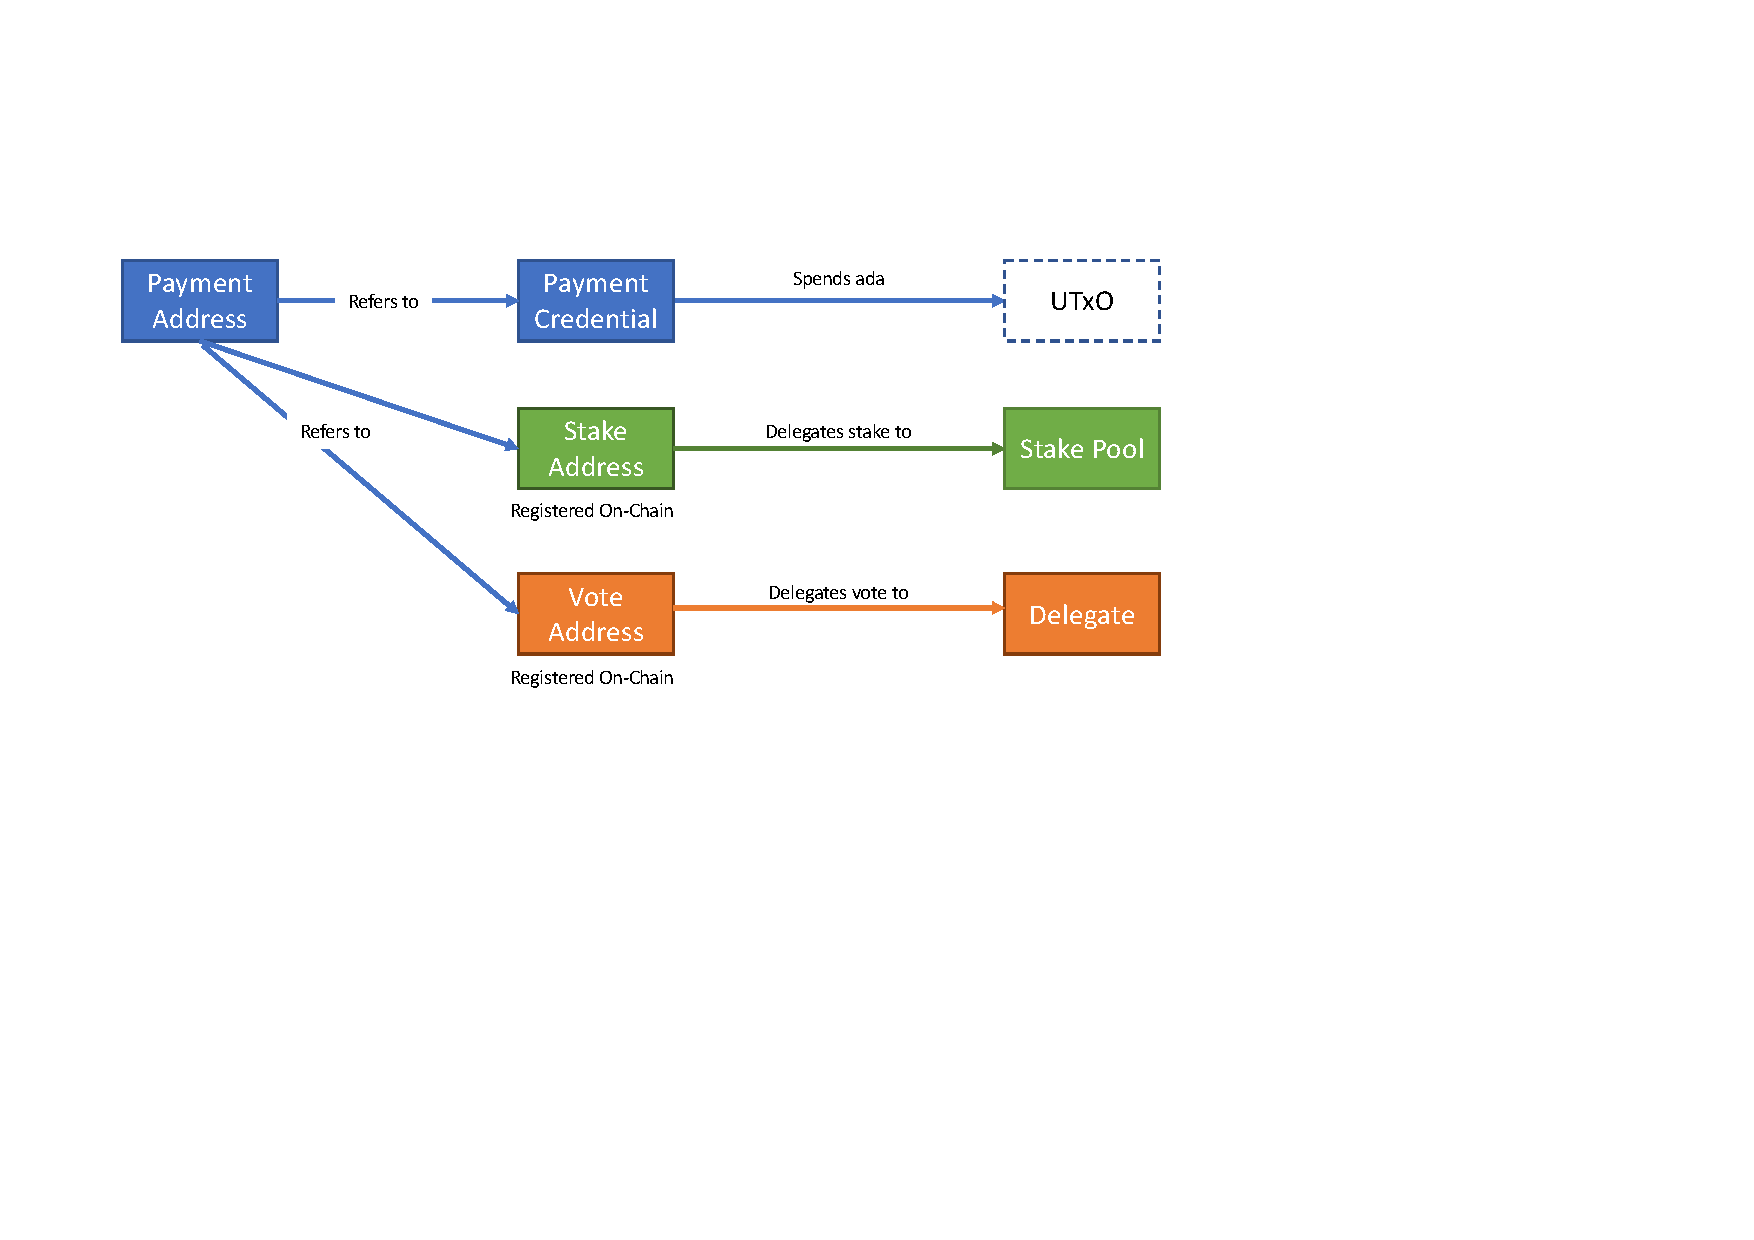
\includegraphics[trim=0 150 0 80,clip,width=\textwidth]{Indirection}
  \caption{Examples of Indirection}
  \label{fig:indirection}
\end{figure*}

\subsubsection*{Voting Indirection}

Figure~\ref{fig:indirection} shows how payment addresses are related to stake and vote addresses.

\begin{figure*}[h]
  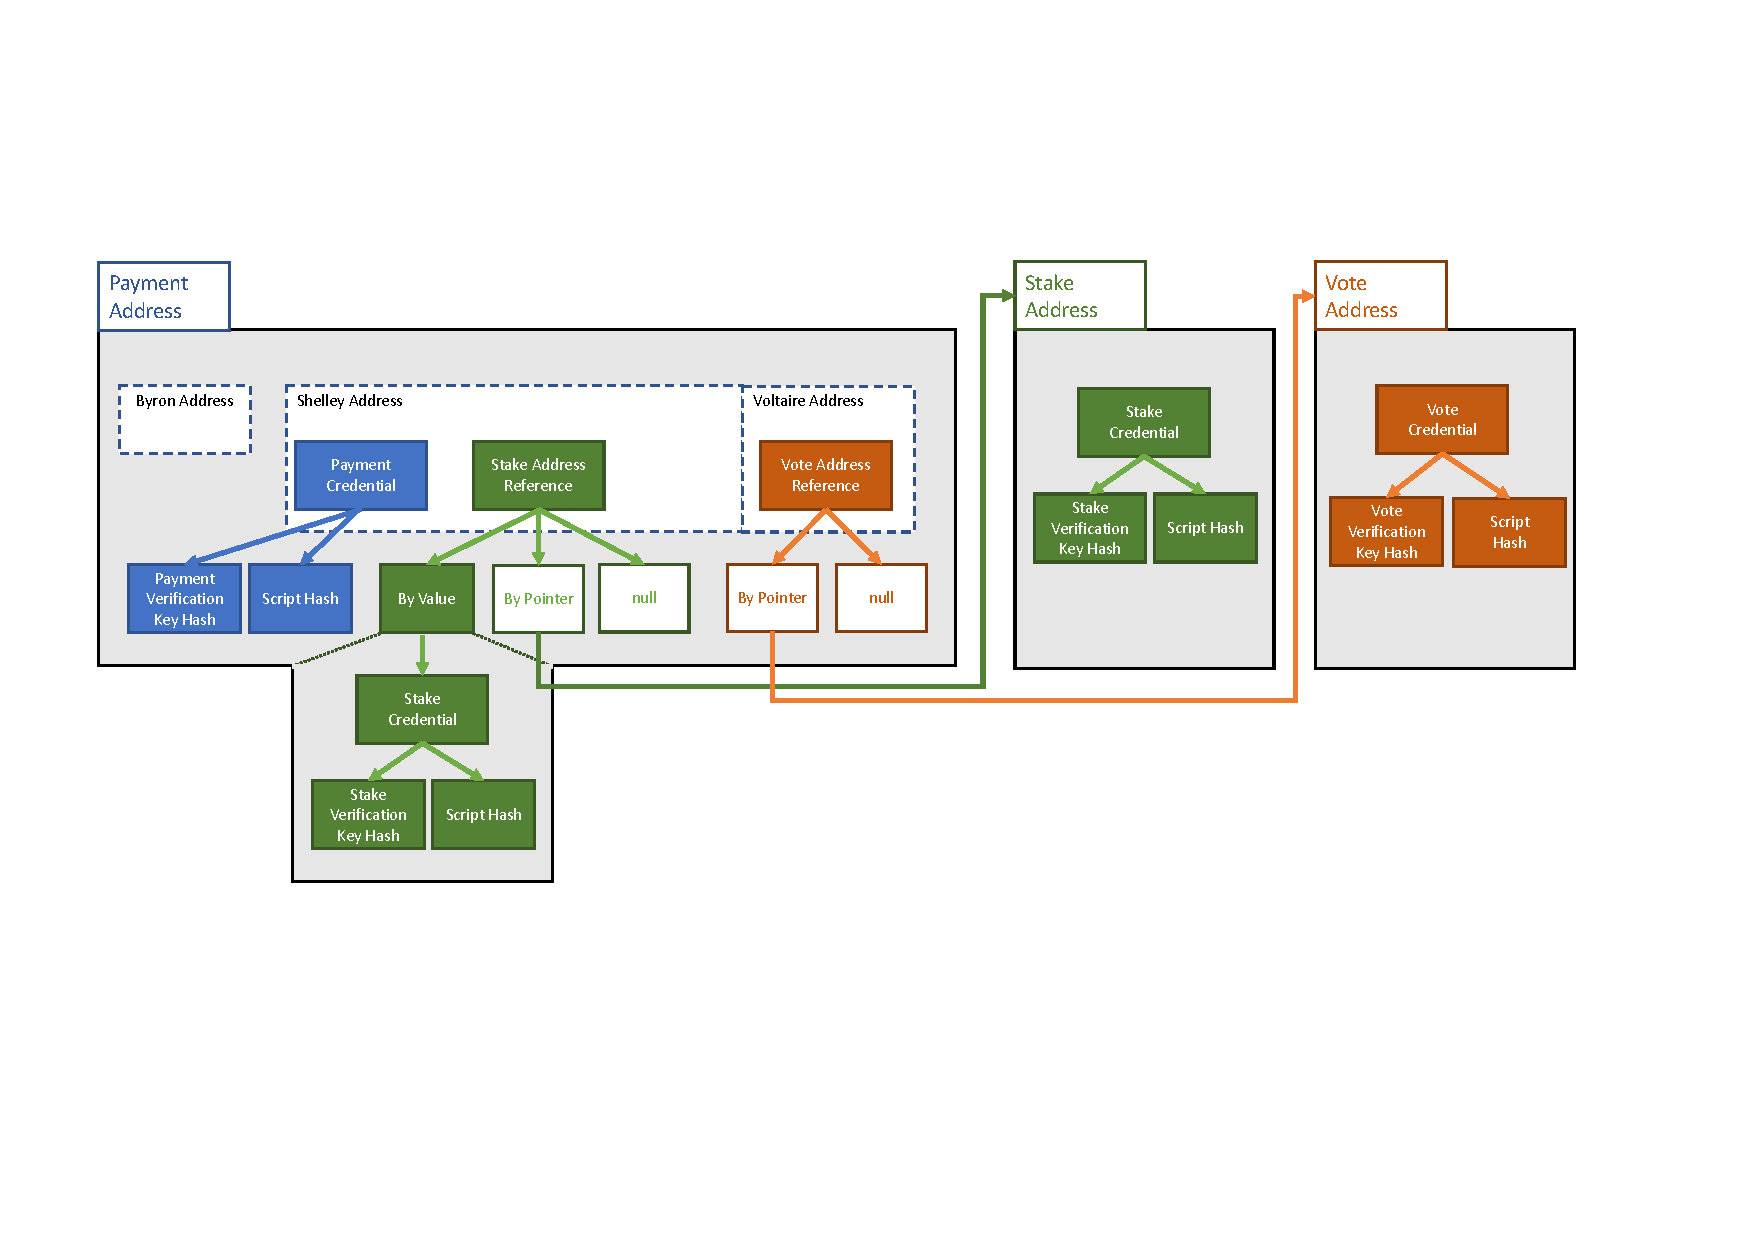
\includegraphics[trim=0 150 0 80,clip,width=\textwidth]{Address-Structure}
  \caption{Payment Stake and Vote Address Structure}
  \label{fig:address-structure}
\end{figure*}

\subsubsection*{Address Structure}

The structure of addresses is shown in Figure~\ref{fig:address-structure} (adapted from the Shelley delegation design document~\cite{..}).
Payment addresses may be either Byron Addresses, Shelley Addresses or Voltaire Addresses.
Voltaire addresses extend Shelley addresses by including a vote address reference in addition to the existing payment credential and stake address
reference fields.  Payment credentials may be either payment verification key hashes or script hashes.  Stake address references may be either
by value (in which case the stake credential is directly embedded in the address), by pointer to the registration transaction, or null (an efficient
form used where payment addresses do not need stake delegation rights).
Stake addresses refer to a stake credential that must either be a stake verification key hash or a script hash.
\khcomment{The Shelley address design looks over-complicated -- stake references could probably be collapsed to just pointers.}
Voltaire extends the Shelley address format by including vote address references.  These must be either by pointer to the registration transaction, or null (an efficient
form used where payment addresses do not need vote delegation rights).
\khcomment{I think the null form might not be used?  In which case we could avoid problems by eliminating it.  However, the vote address would then need either to be optional
or it would be necessary to always register the vote credentials with the payment address.}
Vote addresses refer to a vote credential that is must be a vote verification key hash.
\khcomment{The different levels seem a bit confusing.  An address is presumably a reference to the structure.  But embedded stake credentials won't have an address.  Credentials similarly
seem to always collapse down to the underlying structure (so may be naming artefects that do not really need to exist).}
\khcomment{Should script hashes be allowed as voting credentials?  I would imagine so.}
